\subsection{Proceso Interno 07: Iniciar Simulación}

\subsubsection{Objetivo del Proceso}
Ejecutar integración numérica en REBOUND para:
\begin{itemize}
    \item Generar trayectoria completa del sistema
    \item Almacenar estados temporales
    \item Activar recolección de datos en $t_{\text{vis}} \in t_{\text{vis\_list}}$
    \item Preparar datos para cálculo de LE
\end{itemize}

\subsubsection{Entradas Principales}
\begin{itemize}
    \item \textbf{sim}: Objeto \texttt{Simulation} configurado
    \item $T_{\text{max}} \in \mathbb{R}^+$ (tiempo máximo)
    \item $t_{\text{vis\_list}} \subset [0, T_{\text{max}}]$ (instantes de visualización)
\end{itemize}

\subsubsection{Sub-pasos Secuenciales}
Este apartado es proporcionado para profundizar y describir de forma textual cada paso contenido dentro del diagrama del proceso descrito en la figura~\ref{fig:process_diagram07}
\subsubsection*{1. Inicializar Almacenamiento}
\begin{itemize}
    \item Crear estructuras:
    \begin{itemize}
        \item \texttt{time\_steps} = $[\;]$
        \item \texttt{position\_history} = $[\;]$
        \item \texttt{velocity\_history} = $[\;]$
    \end{itemize}
    \item Capturar estado inicial en $t=0$
\end{itemize}

\subsubsection*{2. Bucle Principal de Simulación}
\begin{enumerate}[label=\textbf{Paso \arabic*:}]
    \item \textbf{Condición}: $\texttt{sim.t} < T_{\text{max}}$
    \item \textbf{Integración}:
    \begin{verbatim}
sim.integrate(sim.t + sim.dt)
    \end{verbatim}
    \item \textbf{Almacenamiento}:
    \begin{itemize}
        \item Actualizar \texttt{time\_steps}
        \item Registrar posiciones/velocidades
    \end{itemize}
    \item \textbf{Verificación Visualización}:
    \begin{equation*}
        \exists t_{\text{vis}} \in t_{\text{vis\_list}} \quad | \quad |\texttt{sim.t} - t_{\text{vis}}| < \epsilon
    \end{equation*}
    \item \textbf{Recolección Condicional}:
    \begin{itemize}
        \item Si coincide: Activar módulo de visualización
        \item Si no: Continuar integración
    \end{itemize}
\end{enumerate}

\subsubsection{Lógica Interna y Decisiones}
\begin{itemize}
    \item \textbf{Control del bucle}: Condición $\texttt{sim.t} < T_{\text{max}}$
    \item \textbf{Tolerancia visualización}: $\epsilon = dt/2$
    \item \textbf{Manejo de errores}: Excepciones REBOUND
    \item \textbf{Almacenamiento}: Registro completo vs.\ muestreo selectivo
\end{itemize}

\subsubsection{Manejo de Datos Específico}
\begin{itemize}
    \item \textbf{Entradas}:
    \begin{itemize}
        \item Estado inicial de \texttt{sim}
        \item Parámetros temporales
    \end{itemize}
    \item \textbf{Intermedios}:
    \begin{itemize}
        \item Estructuras de almacenamiento dinámicas
        \item Estados intermedios del sistema
    \end{itemize}
    \item \textbf{Salida}:
    \begin{itemize}
        \item \texttt{SimulationResult}: $\{\texttt{time\_steps}, \texttt{position\_history}, \texttt{velocity\_history}\}$
    \end{itemize}
\end{itemize}

\subsubsection{Salidas Principales}
\begin{itemize}
    \item \textbf{SimulationResult}: Estructura con:
    \begin{itemize}
        \item Serie temporal completa
        \item Datos de posición/velocidad
        \item Metadatos de ejecución
    \end{itemize}
\end{itemize}

\subsubsection{Interacciones Internas}
\begin{itemize}
    \item \textbf{Con API REBOUND}:
    \begin{itemize}
        \item Llamadas a \texttt{sim.integrate~()}
        \item Acceso a \texttt{sim.particles}
    \end{itemize}
    \item \textbf{Con módulo de visualización}:
    \begin{itemize}
        \item Activación en $t_{\text{vis}}$
        \item Transferencia de datos parciales
    \end{itemize}
    \item \textbf{Con sistema de almacenamiento}:
    \begin{itemize}
        \item Gestión eficiente de grandes datasets
    \end{itemize}
\end{itemize}
\newpage
\subsubsection{Diagrama del Proceso}
\begin{figure}[H]
    \centering
    \adjustbox{max width=\textwidth, max height=0.9\textheight}{%
        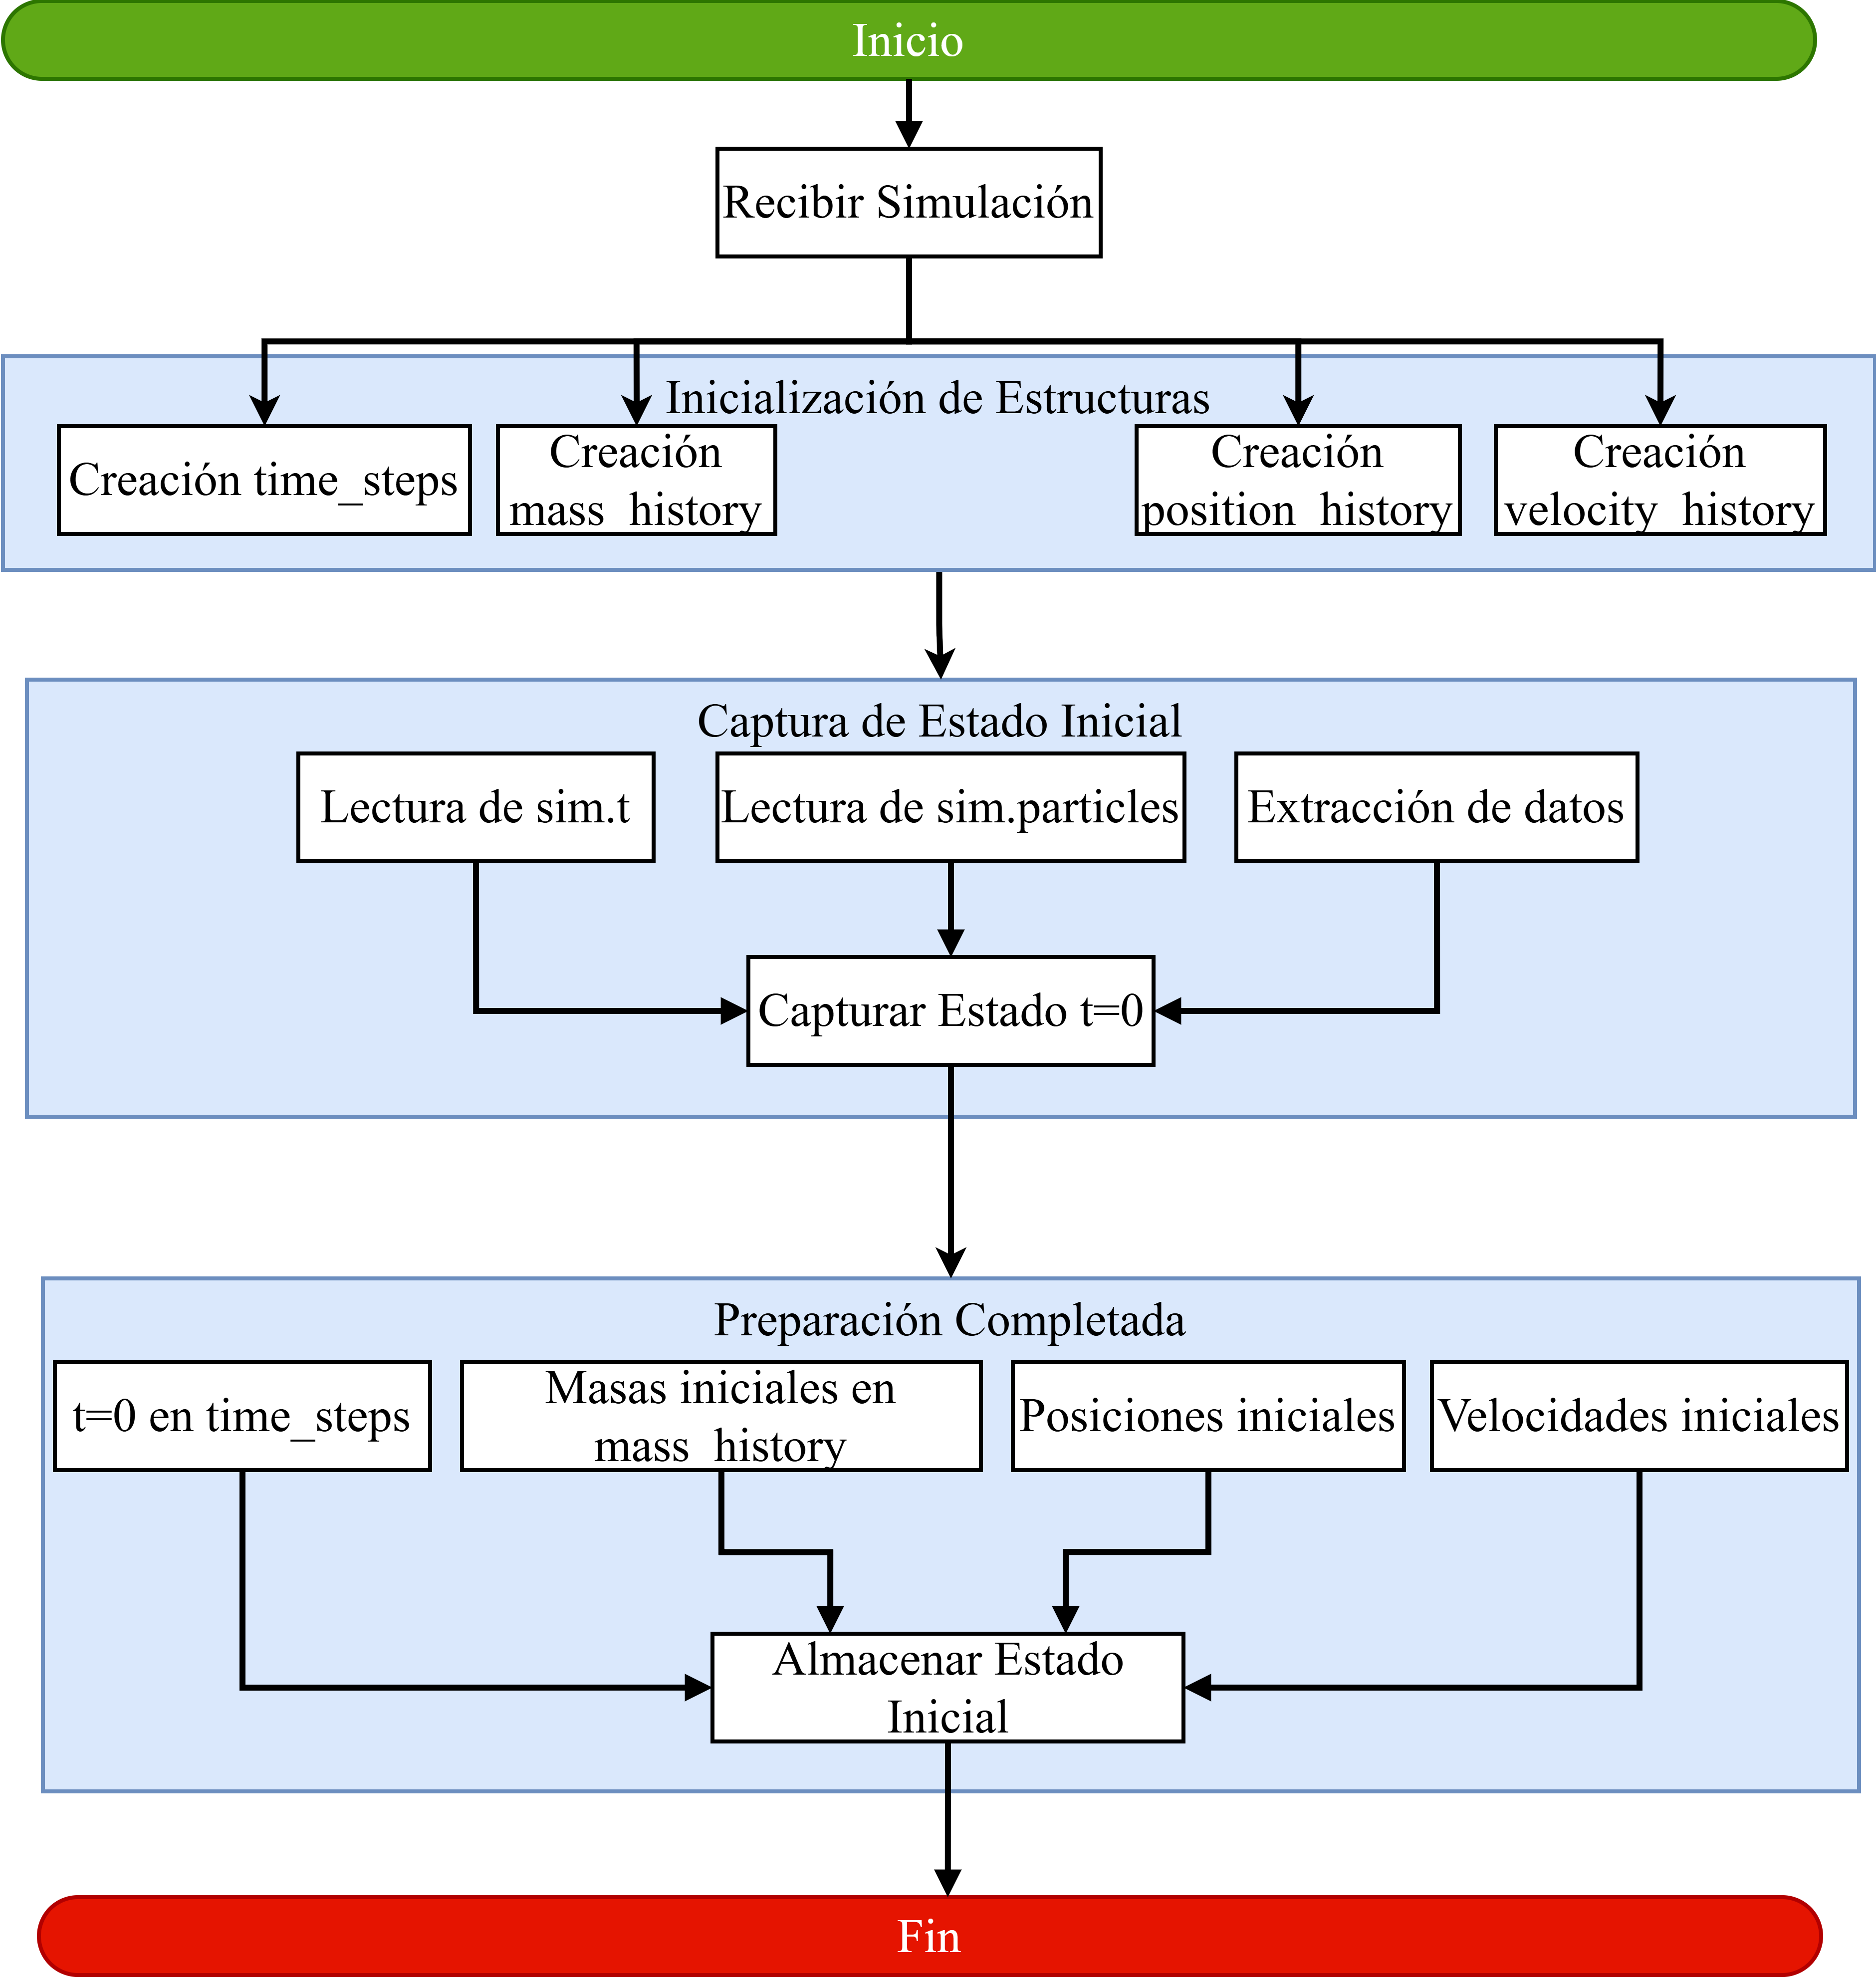
\includegraphics{img/Analisis/DiagramaProcesos/DiagramaProceso07_IniciarSimulacion.png}
    }
        \caption{Diagrama de Proceso Interno 07: Iniciar Simulación}%
    \label{fig:process_diagram07}
\end{figure}
\newpage